\chapter{Présentation de l'entreprise et des missions}
% \chapter{Présentation de l'entreprise}

% \section{Fondateurs}
% \section{Structure juridique}
% \section{Son développement}
% \section{Ses objectifs}
% \section{Ses clients potentiels}
% \section{Les membres}
% \section{Le lieu}

Dans cette partie, on examinera dans un premier temps l'entreprise afin de situer dans quel contexte j'ai effectué mon année en apprentissage. Puis, je décrirais quelles ont été les différentes missions que j'ai effectué, et j'expliquerais pourquoi elles m'ont été demandées.

%mieux vaut un plan en entonnoir
%les clients, les objectifs de l'entreprise, le fondateur, le rachat par spie, les deux parties (infogérance et ...), 
\section{Présentation de l'entreprise}
\subsection{Une société de services}
\paragraph{}
\newacronym{ssii}{SSII}{Société de Services en Ingénierie Informatique}
\newglossaryentry{cloud}{name={cloud computing},description={Concept qui consiste à déporter sur des serveurs distants des stockages et des traitements informatiques traditionnellement localisés sur des serveurs locaux. cf. \url{http://fr.wikipedia.org/wiki/Cloud_computing}}}
\newglossaryentry{infogerance}{name={infogérance},description={C’est l’externalisation de tout ou partie de la gestion et de l’exploitation du SI à un prestataire informatique tiers (SSII). cf. \url{http://fr.wikipedia.org/wiki/Infogérance}}}
APX est une \gls{ssii} fondée par Noël \textsc{Saille}. Son siège social est situé à Saint Cloud (92). Mais, je dépend du centre de services de Rungis (94).
APX est divisée en deux parties : APX Intégration, et APX \Gls{infogerance}.
La première partie est centrée sur le \foreignlanguage{english}{\gls{cloud}}\footnote{Concept qui consiste à déporter sur des serveurs distants des stockages et des traitements informatiques traditionnellement localisés sur des serveurs locaux. cf. \url{http://fr.wikipedia.org/wiki/Cloud_computing}} : elle aide des clients à migrer ses données sur le \foreignlanguage{english}{cloud}.
Tandis que la deuxième partie est plus axée sur le support et la maintenance en vue de répondre à un besoin d'externalisation des entreprises. La partie infogérance (uniquement) a récemment été rachetée par Spie, une autre \gls{ssii}. Je ne mentionnerais donc que Spie dans ce rapport.
J'ai effectué mes missions dans le domaine de l'\gls{infogerance}\footnote{C’est l’externalisation de tout ou partie de la gestion et de l’exploitation du SI à un prestataire informatique tiers (SSII). cf. \url{http://fr.wikipedia.org/wiki/Infogérance}}.
\subparagraph{}
L'un des plus gros contrats d'infogérance de Spie est celui de Disneyland. Je vais donc vous parler de ce client dans la partie qui suit.


\subsection{Un client}
\paragraph{}
Après avoir exprimé une volonté de changement, Disneyland Paris a confié à Spie la maintenance de son parc informatique, auparavant géré par Econocom (une autre \gls{ssii}).
Depuis septembre 2012, c'est donc Spie qui a repris le contrat de Disneyland Paris.
Disneyland ne sous-traite que la partie maintenance et support technique de son service informatique (pour des raisons financières et des raisons de productivité). Spie ne s'occupe donc pas de la partie \foreignlanguage{english}{hotline} et web.
J'ai donc effectué mes missions au sein des locaux de Spie mis à disposition par Disneyland. Ces locaux sont divisés en trois parties : le stock, les bureaux, et l'atelier.
\subparagraph{}
Après vous avoir parlé de la société dans laquelle j'ai évolué, je vais maintenant décrire l'équipe \textbf{avec}, mais aussi \textbf{pour} laquelle, j'ai travaillé.




\subsection{Une équipe}
\paragraph{}

\newacronym{ot}{OT}{Ordres de Travail}
%\newglossaryentry{ot}{name={OT},description={Ordres de Travail}}
\newglossaryentry{dispatcher}{name={dispatcher},description={Personne chargée de recevoir et retransmettre les \gls{ot}}}
Dans la figure~\ref{organigrammeAPX} page~\pageref{organigrammeAPX}, je décris comment l'équipe est organisée.
J'ai travaillé dans une équipe d'environ 20 membres (cf. fig.~\ref{organigrammeAPX}), composée de techniciens de proximité, de techniciens référents, d'une \foreignlanguage{english}{\gls{team}}, d'un logisticien, d'un logisticien intégrateur, et d'un \foreignlanguage{english}{\gls{dispatcher}\footnote{Personne chargée de recevoir et retransmettre les \gls{ot}}}. Le \foreignlanguage{english}{\gls{team}} gère l'équipe de techniciens. Le logisticien gère le stock de matériels informatiques, et le logisticien intégrateur gère les devis d'installations et les factures de réparations (dans le cas ou le matériel n'est plus réparable par nos propres moyens). Il n'y a donc aucun autre développeur dans l'équipe. Seul le logisticien intégrateur possède des compétences en \gls{vba}.
\paragraph{}
\begin{center}
  \begin{figure}[ht]
    \caption{\label{organigrammeAPX} Organigramme de l'équipe}
    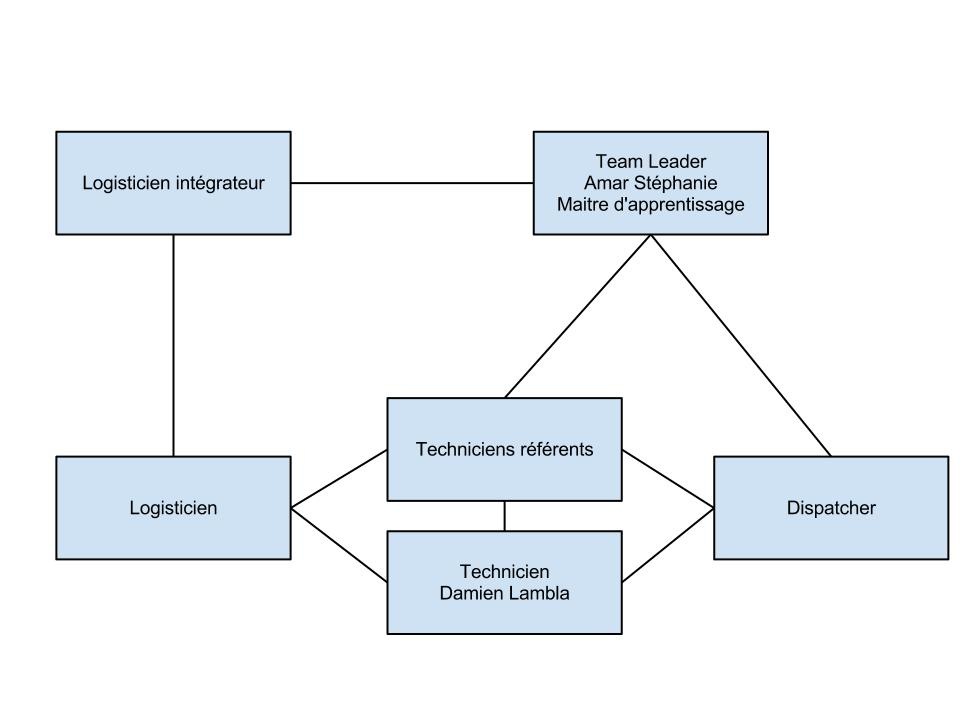
\includegraphics [width=1\textwidth]{images/Organigramme_APX.jpg}
  \end{figure}
\end{center}
